\documentclass[11pt, letterpaper]{article}

% -------------------------------------------------------------------------
% Commands
\usepackage[utf8]{inputenc}
\usepackage{graphicx}
\usepackage{hyperref}
\usepackage{cite}
\usepackage{vmargin}
\usepackage{lipsum}  

\setmargins{2.5cm}                 % margen izquierdo
{1.5cm}                            % margen superior
{16.5cm}                           % anchura del texto
{23.42cm}                          % altura del texto
{10pt}                             % altura de los encabezados
{1cm}                              % espacio entre el texto y los encabezados
{0pt}                              % altura del pie de página
{2cm}                              % espacio entre el texto y el pie de página

% \hyphenation{}

% \hypersetup{colorlinks,%
% 	citecolor=blue,%s
% 	filecolor=blue,%
% 	linkcolor=blue,%
% 	urlcolor=blue%
% }


% -------------------------------------------------------------------------
\title{\textbf{$U_i$ dynamics}}

% -------------------------------------------------------------------------

\date{}
\author{
  % \textbf{Jos\'e A. Pereiro-Morej\'on$^{1,3}$, Roberto Mulet$^{1,2}$} \\
  % \small{1. Group of Complex Systems and Statistical Physics.} \\
  % \small{Physics Faculty, University of Havana, CP 10400. La Habana, Cuba} \\
  % \small{2. Department of Theoretical Physics, }\\
  % \small{Physics Faculty Faculty, University of Havana, CP 10400. La Habana, Cuba} \\
  % \small{3. Biology Faculty, University of Havana, CP 10400. La Habana, Cuba} \\
}

% -------------------------------------------------------------------------
% opening
\begin{document}

\maketitle

\begin{abstract}
	\lipsum[2]
\end{abstract}

Baajskhdbck asdckjs dlajdbcliasd claksdc kjhaskdc \cite{pereiro-morejonInferenceMetabolicFluxes2022}. 
jshdkasjdh fkashdvf kasjdf, such as:

\begin{equation}
  U_i(t+1) = (1-\lambda)U_i(t) + \frac{\Gamma}{N} \sum_j s_j (t)
\end{equation}

\lipsum[2]:

\begin{figure}
	\centering
	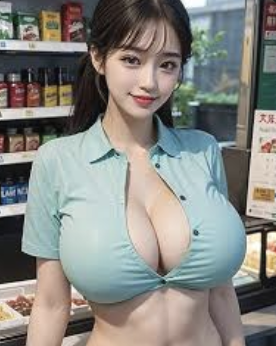
\includegraphics[scale = 0.6]{images/helloWorld.png}
	\caption{
		\textbf{happy life}:
        ascdkjahdc asdcksab dckajshdclsahd cakjshbd cka. 
	}
	\label{fig:label}
\end{figure}

\bibliographystyle{plain}
\bibliography{main}
	
\end{document}
